%
\chapter{Conceitos Fundamentais e Revisão Bibliográfica}
\label{chap:revisaobibliografica}
%\emph{Texto não obrigatório}

\section{Gasolina de Pirólise (\emph{PYGAS})} \label{sec:pygas}
A gasolina de pirólise (\emph{PYGAS - Pyrolysis Gasoline}) é um dos produtos
obtidos no processo de craqueamento a vapor quando da produção de olefinas na
indústria petroquímica. Tipicamente a gasolina de pirólise apresenta curva de
destilação entre 303K e 477K ou mais. Ela é um produto instável (térmica e
químicamente) devido à grande quantidade de compostos insaturados tais como:
monoolefinas, diolefinas conjugadas, estireno e outras espécies mais pesadas e
também reativas \cite{Cheng1986}.
\nomenclature[Z]{PYGAS}{Gasolina de pirólise}
 
A grande quantidade de de compostos insaturados (olefinas e aromáticos) contidos
na gasolina de pirólise lhe fazem um produto interessante, tanto pela
sua alta octanagem quanto pela sua quantidade de aromáticos. Contudo, a
instabilidade (formação de goma, cor) impede sua utilização comercial na forma
como é produzida. Assim, processos de refinamento específicos para essa corrente
são necessários \cite{Derrien1986}.

O esquema de processo a ser utilizado para refinar a gasolina de pirólise
depende do produto final desejado. Para a produção de uma corrente que
comporá a gasolina automotiva, atendendo requisitos tais como estabilidade e
corrosividade, é aplicado a hidrogenação seletiva de diolefinas, também
conhecido como primeiro estágio de hidrogenação. Já se o propósito for a
obtenção de aromáticos, segue-se à hidrogenação seletiva o segundo estágio
de hidrogenação (hidrogenação de olefinas e hidrodessulfurização)
\cite{Derrien1986}.

\section{Reatores de Leito Gotejante} \label{sec:reatorestbr}

\subsection{Definição} \label{sec:definicao}

Na literatura há vários autores que trataram das definições de
reatores catalíticos multifásicos de leito empacotado (PBR - \emph{Packed Bed
Reactors}).
\nomenclature[Z]{PBR}{Reator de leito empacotado}

Segundo \citeonline{Froment2011}, por reatores de leito empacotado multifásicos
entende-se as colunas que possuem recheios catalíticos, e que são destinadas a
promover reações entre compostos presentes em ambas as fases gasosa e líquida.

Assim como \citeonline{Froment2011}, \citeonline{Ancheyta2011} acrescenta à
definição de PBR uma distinção quanto ao regime de escoamento e direção de
escoamento das fases, sendo duas as formas: (i) em regime gotejante, onde a fase
gás é contínua e a fase líquida está distribuída, e a principal resistência a
transferência de massa está na fase gasosa; e (ii) em regime de borbulhamento,
com a fase gás distribuída e a fase líquida contínua, e a principal resistência
a transferência de massa localiza-se na fase líquida.

Os reatores de leito gotejante (TBR - \emph{Trickle Bed Reactor}) compreendem
uma família de PBRs nos quais as fases gasosa e líquida escoam através de um
leito catalítico fixo, sendo eles assim classificados como reatores de leito
fixo (FBR - \emph{Fixed Bed Reactors}). O TBR ainda possui as seguintes
características, segundo \citeonline{Ancheyta2011}.
\nomenclature[Z]{TBR}{Reator de leito gotejante}
\nomenclature[Z]{FBR}{Reator de leito fixo}

\begin{itemize}
\item A fase líquida escoa em sentido descendente (na direção da gravidade),
fluindo sob a forma de filmes, filetes (\emph{rivulet}) e gotículas (e é daí
que vem o nome \textit{gotejante} (\emph{trickle}));
\item A fase gasosa pode escoar tanto ascendentemente (contracorrente à
fase líquida) quando descendentemente (cocorrente à fase líquida)
\end{itemize}

Os PBRs nos quais há escoamento ascendente, tanto da fase gasosa quanto da
fase líquida, opera em regime de borbulhamento, não sendo classificado como
um TBR \cite{Ancheyta2011}.

%A configuração convencional dos TBRs está representada na
%\autoref{fig:configuracoestbr}.

% \begin{figure}[htb]
% \centering 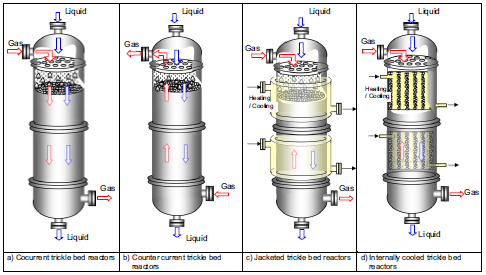
\includegraphics[scale=0.75]{images/Chap2/configuracoestbr.png}
% \caption{Regimes de escoamento em reatores de leito gotejante
 % \cite{Gunjal2005}.}
% \label{fig:configuracoestbr}
 %\end{figure}

\subsection {Regimes de Escoamento}
\label{sec:escoamento}

Um TBR pode ser visualizado como um leito de partículas de catalisador, no qual
o espaço intersticial entre elas formam complexos caminhos e distribuição de
poros. Ao fluir sobre as partículas de catalisador, gás e líquido podem
apresentar diferentes tipos de escoamento ou regimes. Esses regimes de
escoamento dependem da da densidade do leito, da velocidade de escoamento das
fases, do tamanho das partículas de catalisador, das dimensões do reator e das
propriedades físicas dos fluidos \cite{Ranade2011}.

A definição do tipo de escoamento, tanto na fase de projeto quanto na avaliação
de um reator existente, é muito importante pois vários parâmetros
hidrodinâmicos e de transporte são influenciados pelo regime de escoamento. Este
últimos influenciam tanto no dimensionamento dos TBRs quanto nos
equipamentos atrelados a eles, tais como bombas e compressores
\cite{Ranade2011}.

Segundo \apudonline{Ramachandran1983}{Ranade2011}, quatro
diferentes regimes de escoamento foram identificados em TBRs:

\begin{itemize}
	\item Gotejamento (\emph{Trickle flow regime)},
	\item de pulso (\emph{Pulse flow regime)},
	\item Spray (\emph{Spray flow regime)}, e
	\item Borbulhamento (\emph{Buble flow regime)}
\end{itemize}

%Esses regimes de escoamento estão ilustrados na \autoref{fig:regimeescoamento}.

% \begin{figure}[htb]
% \centering 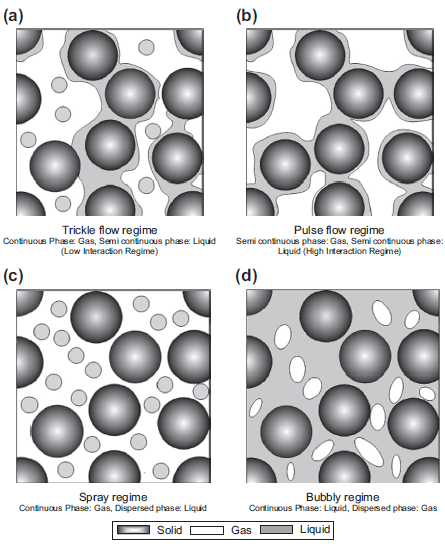
\includegraphics[scale=0.75]{images/Chap2/regimeescoamento.png}
% \caption{Regimes de escoamento em reatores de leito gotejante
 % \cite{Gunjal2005}.}
% \label{fig:regimeescoamento}
% \end{figure}

O escoamento em regime gotejante ocorre em baixo fluxo de líquido e moderado
fluxo de gás. Como já foi dito, o líquido escoa em forma de filmes ou filetes
sobre as partículas do catalisador. Nesse regime de escoamento, a fase contínua
é a gasosa e a fase líquida escoa dispersa. Esse tipo de escoamento também é
chamado de regime de baixa interação \cite{Saroha1996}.

Em fluxo moderado de líquido e gás ocorre o escoamento em regime de pulso,
caracterizado pelo escoamento semicontínuo de ambas as fases. Ante o regime
por gotejamento, o regime de pulso apresenta maior interação entre as fases.
Todavia, esse processo faz com que regiões ricas em gás se alternem com regiões
ricas em líquido \cite{Saroha1996}.

Os outros dois regimes de escoamento encontrados em TBRs são: borbulhamento e
tipo spray. No primeiro, a fase contínua é a líquida, enquanto que a fase gasosa
escoa dispersa; no segundo, a fase contínua é a gasosa, e a fase líquida é
dispersa. Ambos os casos são classificados como regimes de alta interação entre
as duas fases \cite{Saroha1996}.

Os reatores industriais operam com frequência na próximos a transição entre os
regimes gotejante e pulsado. Isso proporciona melhores taxas de transferência de
massa, utilização do catalisador e aumenta a capacidade produtiva
\cite{Ancheyta2011}.

\subsection{Parâmetros Hidrodinâmicos}
\label{sec:parametroshidrodinamicos}

Por natureza, os TBRs possuem uma comlexidade fenomenológica ímpar quando se
trata de seu comportamento hidrodinâmico. Supera em complexidade tanto os FBRs,
onde somente há apenas uma fase escoando pelo leito catalítico, quanto colunas
empacotadas onde não há transferência de massa. 

A compreensão e a previsão, ainda que imprecisamente, dos parâmetros
hidrodinâmicos dos TBRs são as chaves para o projeto e análise desse tipo de
reator. Os parâmetros que serão discorridos a seguir são:

\begin{itemize}
  \item Perda de carga
  \item Retenção de líquido
  \item Molhamento das partícutas de catalisador
  \item Coeficientes de transferência de massa
  \item Dispersões axial e radial de massa
%  \item Transferência de calor em TBRs
\end{itemize}

\subsubsection{Perda de Carga}
\label{sec:perdadecarga}

A capacidade de estimar a perda de carga em TBRs na fase de projeto é de suma
importância. Ela definirá a capacidade de um dos equipamentos mais custosos do
sistema, o compressor que fará a recirculação da fase gasosa. A perda de carga
também é um importante parâmetro a ser acompanhando pelos engenheiros quando o
TBR está em operação.

A perda de carga bifásica ao longo do reator está relacionada com: (i) a
geometria do reator (diâmetro, tamanho e forma do catalisador e geometria dos
internos, tais como prato distribuidor); parâmetros operacionais tais como vazão
de gás e líquido (regime de escoamento); e propriedades das fases (densidade,
viscosidade, tensão superficial etc.). Temperatura e pressão de operação afetam
indireamente a perda de carga através das propriedades do fluido
\cite{Ranade2011}.

Normalmente as equações de perda de carga são definidas em termos de perda de
carga específica $\Delta P/L$, que é definida como a variação da pressão interna
por unidade de comprimento do reator. Em reatores cujo regime é de baixa
interação (regime gotejante de escoamento), a perda de carga tende a ser
pequena. Para regimes de alta interação, a perda de carga pode chegar a alguns
atmosferas por metro \cite{Benkrid1997}.

\nomenclature[G]{$\Delta P/L$}{Perda de carga por unidade de comprimento de
reator \nomunit{kPa/m}}

Segundo \citeonline{Holub1993}, os modelos hidrodinâmicos podem ser
classificados em duas categorias. A primeira categoria lança mão do empirismo
baseado em análise dimensional para produzir correlações de perda de carga e
retenção de líquido. A segunda categoria utiliza equações tipo Ergun
\apud{Ergun1952}{Holub1993}, modificando parâmetros para escoamento bifásico.
Essa abordagem é aplicada especialmente para regimes de escoamento de baixa
interação.

\citeonline{Holub1993}, por exemplo, desenvolveram uma correlação para perda
de carga para TBRs operando em regimes de baixa interação. Já
\citeonline{Benkrid1997} utilizaram dados experimentais  da literatura para
propor modelos simples de perda de carga em TBRs que operam em regimes de alta
interação. Ambos autores citados neste parágrafo também desenvolveram
correlações para retenção de líquido.

Diferentemente de muitos autores, que propuseram equações utilizando dados
experimentais coletados em pressões atmosféricas, \citeonline{Larachi1991}
construiu correlações tanto para perda de carga quanto para retenção de líquido,
em pressões de até $8.1$ MPa.

\subsubsection{Retenção de Líquido}
\label{sec:retencaodeliquido}

A retenção de líquido (\emph{liquid holdup})em um leito de TBR  pode ser
expressada de duas maneiras: (i) retenção total ($\epsilon_L$), definida
como o volume de líquido por unidade de volume de leito e (ii) saturação de líquido
($\beta_L$), definida como o volume de líquido por unidade de volume vazio
(ao invés de volume total de leito). 

A retenção de líquido é composta de duas partes: estática ($\epsilon_{Ls}$) e
dinâmica ($\epsilon_{Ld}$). Por renteção de líquido estática entende-se a porção
de líquido que permanece na superfície das partículas de catalisador após o
leito ser drenado. A fração removida de líquido é definida como retenção
dinâmica \cite{Ranade2011}. Alguns autores utilizam como referência a saturação
de líquido estática ($\beta_{Ls}$) e saturação de líquido dinâmica ($\beta_{Ld}$).

Há algumas ténicas para determinação da retenção de líquido em TBRs. De acordo
com \cite{Benkrid1997}, a técnica mais comum é a da drenagem, já mencionada.
Essa técnica consiste em cessar simultaneamente a alimentação de gás e líquido
no reator (topo), coletando o líquido na saída (fundo). O volume de líquido
drenado significará diretamente $\epsilon_{Ld}$. Outra técnica é consiste em
determinar a massa do reator enquanto seco e em operação, quando gás e líquido
estarão escoando pelo leito catalítico. Esse método levará diretamente a
determinação de $\beta_L$. \cite{Larachi1991} utiliza a distribuição do tempo de
residência para chegar a $\beta_L$.

Vários fatores em TBRs são dependentes da retenção de líquido, tais como fator
de molhabilidade e coefientes de transferência de massa e calor. A retenção de
líquido também determina o tempo de residência de líquido dentro do reator e,
portanto, a conversão dos reagentes \cite{Ranade2011}.

\nomenclature[G]{$\epsilon_{L}$}{Retenção total de líquido}
\nomenclature[G]{$\epsilon_{Ls}$}{Retenção estática de líquido}
\nomenclature[G]{$\epsilon_{Ld}$}{Retenção dinâmica de líquido}
\nomenclature[G]{$\beta_L$}{Saturação de líquido}
\nomenclature[G]{$\beta_{Ls}$}{Saturação de líquido estática}
\nomenclature[G]{$\beta_{Ld}$}{Saturação de líquido dinâmica}

\subsubsection{Molhamento das Partículas de Catalisador}
\label{sec:molhamento}

Dentre os difersos tipos de reatores multifásicos, o molhamento das partículas
de catalisador é um fenômeno exclusivo em TBR. Levando-se em conta que, em um
TBR, a fase líquida escoa de forma não uniforme, a determinação do molhamento do
catalisador é uma tarefa bastante difícil \cite{Ranade2011}

Na literatura são definidos dois tipos de molhamento. \citeonline{Colombo1976}
os descreve assim:

\begin{itemize}
	\item Molhamento interno ou enchimento de poro: é o volume de líquido dentro
	dos poros do catalisador. Como as partículas de catalisador são quase sempre
	porosas, o molhamento interno é considerado total devido ao efeito de
	capilaridade.
	\item Molhamento externo: é a área externa à partícula de catalisador
	efetivamente em contato com o líquido que escoa. Praticamente toda a
	transferência de massa entre o líquido presente nos poros do catalisador e o
	líquido que escoa por sobre as partículas ocorre nessa área.
\end{itemize}

Isto posto, a \emph{eficiência de molhamento} ($\eta_{CE}$) deriva da definição
de molhamento externo. Em outras palabras, ela é definida como sendo a
porcentagem da área superficial externa do catalisador que está efetivamente em
contato com o líquido que escoa \cite{Schwartz1976}.

De acordo com a literatura disponível, a medição da eficiência de molhamento
pode ser direta e indireta. Entre os métodos diretos estão técnicas
fotográficas, método de injeção de corante, imagem de ressonância magnética,
entre outros \apud{Sederman2001}{Ranade2011}. Já os métodos indiretos são
aplicáveis a unidades industriais além de possuirem melhor custo-benefício
\cite{Ranade2011}. \citeonline{Colombo1976} e \citeonline{Schwartz1976}, por
exemplo, utilizaram métodos baseados tanto em taxa de reação quanto em
transferência de massa para determinar a eficiência de molhamento.

\nomenclature[G]{$\eta_{CE}$}{Eficiência de molhamento}

\subsubsection{Coeficientes de Transferência de Massa}
\label{sec:coeficientes}

Em reatores com escoamento gotejante não há um mecanismo severo de mistura como
em outros tipos de escoamento (tanques de mistura ou regimes de alta interação).
Logo, as taxas de transferência de massa são menores em TBRs do que em outros
reatores, podendo limitar a taxa das reações. Os três tipos de taxas de
transferência de massa relevantes nos TBRs são: gás-líquido, líquido-sólido e
gás-sólido \cite{Ranade2011}.

A ocorrências desses tipos de transferência de massa dependerá da eficiência de
molhamento e da retenção de líquido. Em reatores com eficiência de molhamento
próxima a totalidade, por exemplo, desconsidera-se a transferência de massa
gás-sólido \cite{Ranade2011}.

\subsubsection{Dispersões Axial e Radial de Massa}
\label{sec:dispersoes}

As dispersões axial e radial são dois fenômenos que ocorrem em TBRs,
desviando-os da idealidade de escoamento contida no conceito de PFR (PFR -
\emph{Plug-flow Reactor}).

\nomenclature[Z]{PFR}{Reator de escoamento empistonado}

A dispersão radial está diretamente ligada a distribuição de líquido na entrada
do reator. Esse efeito possui uma quantidade pequena de estudos na literatura.
Isso acontece porque, em reatores industriais, a instalação de distribuidores de
carga na entrada dos TBR (topo) promove uma distribuição radial de massa
uniforme. A razão entre o diâmetro do reator e diâmetro da partícula de
catalisador ($D_R/d_p$) tem se mostrado influente na distribuição radial de
massa \cite{Saroha1998}. \citeonline{Al-Dahhan1994}, por exemplo, sugerem que,
mesmo para reatores em alta pressão, um valor de $D_R/d_p > 20$ minimiza a má
distribuição de líquido.

Diferente do que ocorre com a dispersão radial, a dispersão axial é um fenômeno
amplamente estudado, com várias referências na literatura. Esse fenômeno está
ligado a retromistura de líquido dentro do leito catalítico e está relacionado
com a razão entre o comprimento do reator e diâmetro da partícula de catalisador
($L_R/d_p$) \cite{Ancheyta2011}.

\nomenclature{$D_{R}$}{Diâmetro do reator \nomunit{m}}
\nomenclature{$L_{R}$}{Comprimento total do reator \nomunit{m}}
\nomenclature{$d_{p}$}{Diâmetro da partícula de catalisador \nomunit{m}}

Alguns fatores que contribuem na distribuição de líquido e na retromistura são:
capilaridade, zonas-morta, molhamento parcial e caminhos preferenciais
\cite{Ranade2011}.

\subsection{Reações Químicas em TBR} \label{sec:reacoestbr}
 
As reações químicas em FBRs possuem uma complexidade maior ante as reações
homogêneas justamente pela presença de um catalisador sólido. A superfície
de uma partícula de catalisador, em toda a sua complexidade, se apresenta
como o local onde as reações ocorrem. Além disso, fenêmenos de transporte
de massa podem influenciar na taxa global da reação \cite{Froment2011}. 

Sendo assim, os passos envolvidos em uma reação química, na superfície de um
catalisador, para um reator cujo escoamento é monofásico são \cite{Froment2011}: 

\begin{enumerate}
\item Transporte dos reagentes do seio do fluido para a superfície
do catalisador;
\item Transporte dos reagentes nos poros do catalisador;
\item Adsorção dos reagentes no sítio catalítico;
\item Reação química entre os átomos ou moléculas;
\item Dessorção dos produtos;
\item Transporte dos produtos da reação dos poros de volta à
superfície do catalisador;
\item Transporte dos produtos da superfície das partículas para o seio do
fluido.
\end{enumerate} 

Segundo \apud{Ramachandran1983}{Ranade2011}, para os TBRs onde as partículas de
catalisador estão completamente molhados (velocidade espacial de líquido $>0.5
cm/s$), os passos apontados por \citeonline{Froment2011} ganham novas etapas,
como segue:

\begin{enumerate}
\item Transporte dos reagentes presentes na fase gasosa para o seio da
fase líquida;
\item Transporte dos reagentes presentes na fase líquida para a superfície do
catalisador;
\item Transporte dos reagentes nos poros do catalisador;
\item Adsorção dos reagentes no sítio catalítico;
\item Reação química entre os átomos ou moléculas;
\item Dessorção dos produtos;
\item Transporte dos produtos da reação dos poros de volta à
superfície do catalisador;
\item Transporte dos produtos da superfície das partículas para o seio da fase
líquida;
\end{enumerate} 

Ainda pode haver mais um passo em que um dos produtos, se termodinamicamente
favorável, passasse para a fase gasosa. Em reatores de hidrotratamento de
diesel, por exemplo, o $H_2S$ produto descola-se parcialmente para a fase
gasosa, diminuindo a pressão parcial de hidrogênio. O hidrogênio nesse caso é
o reagente em excesso \cite{Ancheyta2011}.

Entretanto, muitos TBRs comerciais operam com velocidades superficiais de
líquido baixas $(<0.5 cm/s)$. Isso faz com que o regime de escoamento seja
classificado como de baixa interação e, consequentemente, não molha
completamente a superfície das partículas. Nesse caso, a taxa de reação
dependerá da fase em que está o reagente limitante \cite{Ranade2011}.

\section {Modelagem de Reatores de Leito Fixo} \label{sec:modelagemreatores}

Várias formas de modelagem de FBRs podem ser encontradas na literatura.
Segundo \citeonline{Froment2011}, os modelos podem ser categorizados em dois
grandes grupos: pseudo-homogêneos e heterogêneos. Por modelos pseudo-homogêneos
entende-se aqueles que não fazem distinção entre as fases, i.e., não considera a
presença do catalisador. Em se tratando de um TBR, não há também distinção entre
as fases líquida e gasosa. Já modelos heterogêneos distinguem, no mínimo, as
partículas de catalisador como uma fase distinta.

Ainda de acordo com \citeonline{Froment2011}, tanto os modelos pseudo-homogêneos
quanto os heterogêneos podem ser classificados em unidimensionais e
bidimensionais. Os modelos bidimensionais consideram gradientes radiais de massa
e/ou calor. Já modelos unidimensionais consideram a idealidade de escoamento
empistonado, podendo ou não contemplar a dispersão axial.

Os modelos também podem ser de treinamento (aprendizagem) ou de predição.
Modelos de treinamento são baseados em redes neurais, ao passo que modelos de
predição podem ser divididos em estocásticos e determinísticos. Os modelos
estocásticos possuem a característica de considerar o arranjo aleatórios das
partículas de catalisador e dos espaços vazios no leito do reator
\cite{Ancheyta2011}. 

Dentro da categoria de modelos determinísticos há os modelos contínuos e modelos
discretos. Os modelos contínuos contém um conjunto de equações diferenciais com
uma ou mais variáveis independentes, onde todas devem ser resolvidas
simultaneamente. Já nos modelos discretos o reator é representado por um número
finito de elementos de reator \cite{Ancheyta2011}. Diferentemente dos modelos
contínuos (equações diferenciais), a modelagem discreta encarrega-se de resolver
equações algébricas para o caso de estado estacionário, ou equações diferenciais
ordinária quando se trata de simulação dinâmica \cite{Schnitzlein1987}.

\citeonline{Deans1960} são apontados como os primeiros a construir um modelo
baseado em estágios discretos em TBRs, chamado de \emph{rede de células} por
alguns autores (\citeonline{Schnitzlein1987} e \citeonline{Ancheyta2011}, por
exemplo). Nesse trabalho, o método de modelagem por rede de células foi aplicado
para estudar os fenômenos de dispersão axial e radial. Segundo
\citeonline{Schnitzlein1987}, independente do arranjo das células, a descrição
do sistema reacional dentro de cada célula pode ser pseudo-homogêneo ou
heterogêneo.

Outra abordagem de modelagem discreta são os modelos \emph{baseados em
estágios}. Nesses modelos há a utilização da \emph{abordagem baseada em taxa}.
Esta última é fundamentada na aplicação direta dos fenômenos de difusão,
transferência de calor e dos efeitos de interação multicomponente no cálculo de
cada segmento (estágio) \cite{Jakobsson2004}. Foi com essa abordagem que
\citeonline{Jakobsson2004} modelou reatores de hidrotratamento de diesel, em
suas operações contracorrente e cocorrente.

\section {Modelagem e Simulação de Hidrogenação Seletiva de Gasolina de Pirólise}
\label{sec:hidrogenacaopygas}

O primeiro estágio de hidrogenação da gasolina de pirólise, também conhecido
como hidrogenação seletiva, foi estudado por alguns autores encontrados na
literatura, incluindo algumas avaliações de resposta dinâmica. A seguir serão
apresentadas algumas informações publicadas.

\subsection{Descrição Geral do Processo} \label{sec:descricaogeral}

A gasolina de pirólise é hidrogenada em um reator tipo TBR, onde o catalisador
pode ser de paládio ou níquel suportado em alumina. Normalmente, o reator possui
ao menos dois leitos. Devido a exotermicidade das reações, há uma injeção de
quench líquido entre os leitos, composta de produto hidrogenado resfriado, que
serve para controlar a temperatura do segundo leito e evitar o coqueamento sobre
a superfície do catalisador. O produto hidrogenado pode também diluir a carga do
reator, retardando o processo de desativação já mencionado
\cite{Cheng1986,Derrien1986,Arpornwichanop2002,Rojas2014a}.

\subsection{Cinética das Reações} \label{sec:cineticadasreacoes}

As duas principais reações que ocorrem em reatores de hidrogenação de gasolina
de pirólise são: conversão de diolefinas em olefinas e olefinas em parafinas, e
de forma sequencial. Como já mencionado, o grau de hidrogenação dependerá da
utilização final da corrente hidrogenada \citeonline{Cheng1986}.

\citeonline{Cheng1986} publicaram valores de constantes cinéticas para a
hidrogenação de gasolina de pirólise, agrupando os compostos em diolefinas,
olefinas e parafinas. Além disso, as reações foram tratadas como irreverssíveis.
A equação \autoref{eq:hidrogenacao} mostra o que foi descrito.

\begin{equation}
Diolefinas -> Olefinas -> Parafinas
\label{eq:hidrogenacao}
\end{equation}

Enfim, \citeonline{Cheng1986} apurou as constantes cinéticas de assummindo que
as reações fossem de pseudo-primeira ordem, ou seja, a concentração de
hidrogênio na fase líquida foi tida como constante.

\citeonline{Authayanun2008} publicaram uma simulação de um reator de
hidrogenação parcial de gasolina de pirólise. Um dos objetivos deste trabalho
foi a determinação das constantes de velocidade específicas, assumindo as
mesmas considerações feitas por \citeonline{Cheng1986}, exceto que as as
reações fossem de pseudo-primeira ordem, i.e., a concentração de hidrogênio
compôs a equação da velocidade das reaçãos. Além disso, foi adicionado um termo
de adsorção à cinética de reação das olefinas, uma vez que a reação destas é
fortemente influenciada pela concentração de diolefinas, como demonstrado
recentemente por \citeonline{Zhou2010}. \citeonline{Arpornwichanop2002} trataram
as reações de hidrogenação da mesma forma que \citeonline{Authayanun2008} as
fizeram.

\citeonline{Rojas2014a} e \citeonline{Mostoufi2005a} utilizaram as mesmas
premissas apresentadas por \citeonline{Cheng1986}, contudo não agrupando os
compostos em diolefinas, olefinas e parafinas; as reações consideradas estavam
entre aquelas apresentadas por \citeonline{Hanika1999}.

\subsection{Considerações sobre Propriedades Físicas e Equilíbrio Líquido-Vapor}
\label{sec:consideracoeselv}

Como já mencionado na seção \autoref{sec:modelagemreatores}, modelos de reatores
determinísticos contínuos necessitam resolver um sistema de equações
diferenciais para obter os resultados de simulação. Nesses modelos, a inserção
de equações que descrevam o equilíbrio líquido-vapor (ELV)) é trabalhoso. Em
TBRs de hidrotatamento de diesel, segundo \citeonline{Ancheyta2011}, as premissa
de (i) fase gasosa em excesso, cuja composição é próxima a de hidrogênio puro, e
(ii) de que os compostos em fase líquida não mudam de fase, facilitam os
cálculos por essa abordagem.

Nos estudos realizados por \citeonline{Authayanun2008},
\citeonline{Arpornwichanop2002}, \citeonline{Arpornwichanop2008} e
\citeonline{Mostoufi2005a} as propriedades das fases gasosa e líquida foram
mantidas constantes ao longo de todo o reator, inclusive a concentração de
hidrogênio na fase líquida. A consequência disso é que, nesses trabalho, os
efeitos de aquecimento tanto na taxa da reação quanto nos fenômenos
hidrodinâmicos permanece desconhecida.

Entretanto, \citeonline{Rojas2014a}, em sua modelagem de um reator de
gasolina de pirólise, modela o ELV atraves de um \emph{flash}
adiabático, utilizando a abordagem $\phi-\phi$. Isso foi feito porque um dos
objetivos desse trabalho foi comparar diferentes modelos equações de estado (e
seus parâmetros) quanto a solubilidade de hidrogênio em gasolina de pirólise. A
base termodinâmica da solubilidade de hidrogênio em gasolina de pirólise
utilizada por \citeonline{Rojas2014a} está nos trabalhos de
\citeonline{Rojas2014a}, que é uma extensão do estudo feito por
\citeonline{Zhou2006}.
\nomenclature[Z]{$ELV$}{Equilíbrio Líquido-Vapor}

\subsection{Hidrodinâmica} \label{sec:hidrodinamica}
Todos os trabalho encontrados sobre hidrogenação parcial de gasolina de pirólise
classificam o reator como um TBR \cite{Arpornwichanop2002, Authayanun2008,
Mostoufi2005a, Arpornwichanop2008, Rojas2014a}. 

O trabalho de \citeonline{Rojas2014a} desta dos demais autores citados por
considerar o regime de escoamento do reator como sendo do tipo borbulhamento,
ainda que ambas as fases estejam em escoamento descendente. Assim, algumas
equações hidrodinâmicas usadas são diferentes das utilizadas pelos demais
trabalhos.

\subsection{Transferência de Massa} \label{sec:transferenciamassa}

Sobre o fenômeno de transferência de massa do sistema difusão-reação, 
os autores adotaram posturas conforme as respectivas abordagens cinéticas.

Assim, o grupo de autores que agrupou os compostos em diolefinas, olefinas e
parafinas \cite{Arpornwichanop2002, Authayanun2008} e, ainda, que considerou o
hidrogênio na cinética da reação, também tratou da difusão deste compoposto da
fase gasosa até a superfície do catalisador. 

Em contrapartida, \citeonline{Rojas2014a} e \citeonline{Mostoufi2005a}, por
terem utilizado como base o trabalho de \citeonline{Hanika1999} para a cinética
das reações, consideraram a fase gasosa em grande excesso e, portanto,
neglicenciaram a resistência a transferência de massa na fase gasosa.
Logo, segundo esses autores, a resistência a transferência de massa influente
está na fase líquida (interface líquido-sólido).

\subsection{Abordagens de Modelagem} \label{sec:abordagensmodelagem}

Os pesquisadores que publicaram trabalhos sobre hidrogenação de gasolina
de pirólise, seja a hidrogenação parcial, seja de hidrogenação total, modelaram
os reatores utilizando modelos determinísticos contínuos. A diferença entre
eles fica a cargo do método númerico aplicado. Vale destacar que no caso de
\citeonline{Rojas2014a}, foi elaborado um intrincado algoritmo para a resolução
do reator, e que ainda utilizou de simulador comercial para o cálculo de ELV.

Não foi encontrado qualquer artigo que utilizasse a modelagem por rede de
células para o processo de hidrogenação de gasolina de pirólise.

%\section{Considerações Finais} \label{sec:consideracoesfinais}


